%%%%%%%%%%%%%%%%%%%%%%%%%%%%%%%%%%%%%%%%%%%%%%%%%%%%%%%%%%%%%%%%%%%%%%%%%%%%%%%
% Chapter 3: Recursos y herramientas
%%%%%%%%%%%%%%%%%%%%%%%%%%%%%%%%%%%%%%%%%%%%%%%%%%%%%%%%%%%%%%%%%%%%%%%%%%%%%%%

%+++++++++++++++++++++++++++++++++++++++++++++++++++++++++++++++++++++++++++++++
En este capítulo se hablará tanto del hardware como del software utilizado para
realizar el proyecto. A grandes rasgos se integrará la PlayStation Camera en el
sistema Perenquén, utilizando el framework ROS para el funcionamiento de ambos.


%++++++++++++++++++++++++++++++++++++++++++++++++++++++++++++++++++++++++++++++
\section{Playstation Camera}
\label{3:sec1}
%%%%%%%%%%%%%%%%%%%%%%%%%%%%%%%%%%%%%%%%%%%%%%%%%%%%%%%%%%%%%%%%%%%%%%%%%%%%%%%%
% Chapter 3: Recursos y herramientas
%%%%%%%%%%%%%%%%%%%%%%%%%%%%%%%%%%%%%%%%%%%%%%%%%%%%%%%%%%%%%%%%%%%%%%%%%%%%%%%%

%+++++++++++++++++++++++++++++++++++++++++++++++++++++++++++++++++++++++++++++++
% \section{PlayStation Camera}
% \label{3:sec:1}

% https://en.wikipedia.org/wiki/PlayStation_Camera
% https://blog.es.playstation.com/2013/10/30/ps4-las-preguntas-ms-frecuentes-que-se-te-puedan-ocurrir/#sect6

PlayStation Camera es una cámara utilizada por PlayStation 4 como accesorio. Fue
lanzada al mercado en 2013 coincidiendo con el lanzamiento de la consola, aunque
vendiendose como un accesorio a parte a un precio recomendado de 59.99\$.

\begin{wrapfigure}{l}{0.5\textwidth}
  \vspace{-20pt}
  \begin{center}
    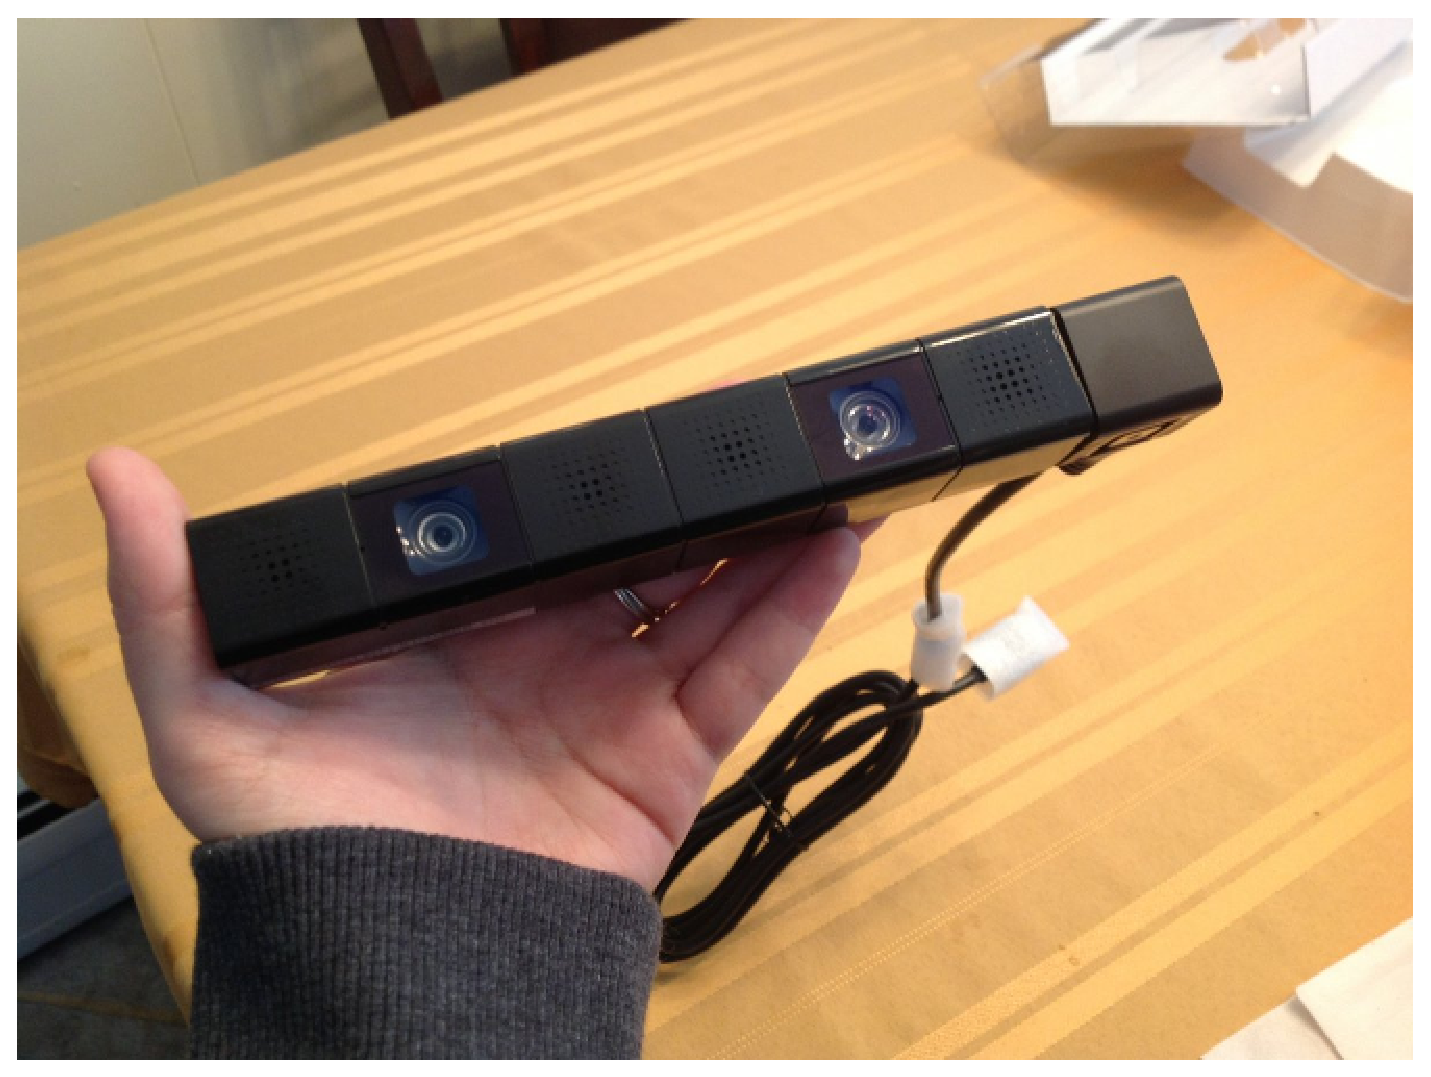
\includegraphics[width=0.48\textwidth]{images/cap3/PlaystationCamera.eps}
  \end{center}
  \vspace{-20pt}
  \caption{PlayStation Camera}
  \vspace{-10pt}
  \label{fig:PlayStation-Camera}
\end{wrapfigure}

Esta camára esta pensada para poder controlar la consola sin necesidad de
utilizar el mando tradicional. Los usuarios de PS4 pueden iniciar sesión
haciendo uso de las características de reconocimiento facial. Tambien permite
utilizar los movimientos del propio cuerpo para moverse por los menús del
sistema y utilizar la voz para realizar acciones gracias al micrófono
incorporado. Playstation Camera también es compatible con otros accesorios de
PlayStation 4 como PlayStation Move (sistema de control por movimiento) para una
navegación más precisa.

Aunque el objetivo principal de PlayStation Camera es su integración en los
vidoejuegos, para conseguir mayor inmersión: control de movimiento, comandos de
voz y tecnología de realidad aumentada.

%+++++++++++++++++++++++++++++++++++++++++++++++++++++++++++++++++++++++++++++++
\subsection{Historia}
Los orígenes de PlayStation Camera vienen desde 1999 cuando Sony empezó a
investigar sobre visión artificial y el uso de reconocimiento de gestos mediante
una cámara para incorporar esta tencnología en los videojuegos. Finalmente en
2003 se lanzaría EyeToy, una cámara que tuvo un notable éxito para PlayStation
2. En 2007, tras la salid de PlayStation 3, se lanzó al mercado una
actualización de esta cámara con el nombre de PlayStation Eye, la cual permitía
capturar imágenes a una mayor resolución y una tasa de fotogramas por segundo
superior.

Mientras que EyeToy y Playstation Eye compartían el mismo concepto, no fue hasta
el lanzamiento de Kinect por parte de Microsoft en 2010, cuando se pudo ver una
evolución real en este tipo de accesorios de entretenimiento. Kinect se basó en
una cámara RGB que contaba con sensores de profundidad, múltiples micrófonos  un
procesador independiente de la consola. Kinect permitía captura de movimiento en
3D, reconocimiento facial y reconocimiento de voz.

Kinect fue un éxito de ventas y obtuvo muchos elogios por parte de la crítica,
pero no en el plano de los vidoejuegos, si no de la investigación. Microsoft
decidió lanzar un SDK oficial para el desarrollo en Windows en base al interés
que existía, para proyectos de todo tipo.

Playstation Camera ha tomado nota de Kinect para ofrecer un producto con las
mismas ventajas de Kinect, aunque utilizando tecnología esteroscópica y
características más modestas para ser una alternativa económica a Kinect.

%+++++++++++++++++++++++++++++++++++++++++++++++++++++++++++++++++++++++++++++++
\subsection{Especificaciones técnicas}
% http://www.psdevwiki.com/ps4/PlayStation_4_Camera

PlayStation Camera cuenta con un chip OV580 encargado de sincronizar las dos
cámaras. Cada cámara cuenta con un sensor de imagen OV9713, mientras que el chip
que controla el sonido es el AK5703. La configuración inicial de la cámara se
almacena en una memoria EEPROM 4g51A.

\begin{minipage}{\linewidth}
    \centering
    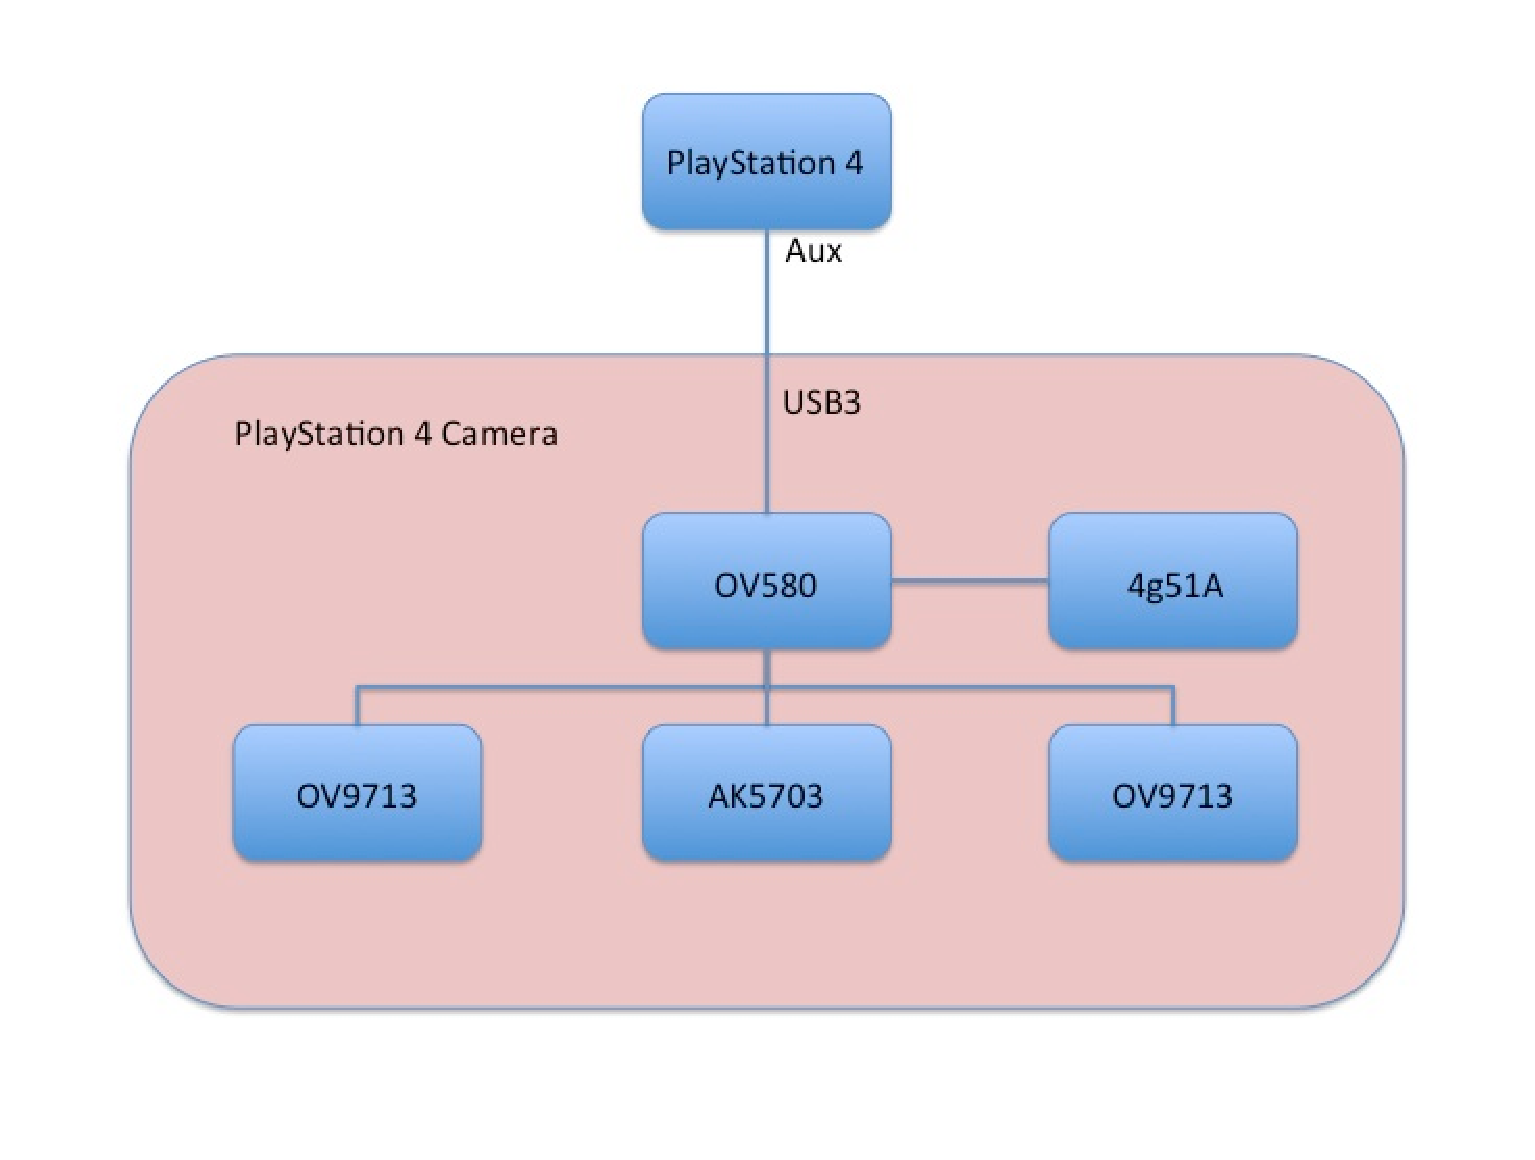
\includegraphics[width=0.9\textwidth]{images/cap3/PlaystationCameraDiagrama.eps}
    \captionof{figure}{Diagrama de PlayStation Camera}
    \label{fig:Playstation-Camera-Diagram}
\end{minipage}

Por su parte ña cámara cuenta con varios ajustes programables: exposición,
balanceo de blancos, gama, saturación, contraste, nitiddez y tono.

%+++++++++++++++++++++++++++++++++++++++++++++++++++++++++++++++++++++++++++++++
\begin{table}[!ht]
\begin{center}
\begin{tabular}{|p{60mm}|p{100mm}|} \hline 
\textbf{Nombre} & \textbf{Descripción} \\ \hline
Dimensiones
&
186mm x 27mm x 27mm
\\
\hline

Peso
&
183 gramos
\\
\hline

Conexión
&
USB 3.0 propietario
\\
\hline

Rango de captura
&
+30cm
\\
\hline

Campo de visión (FOV)
&
85º
\\
\hline

Apertura
&
f/2.0
\\
\hline

Formato de vídeo
&
RAW16/RAW8, YUV442/YUV8
\\
\hline

Profundidad de color
&
12-bit (4096 colores)
\\
\hline

Resolución
&
1280x800 @60FPS,
640x400 @120FPS,
320x200 @240FPS,
160x100 @240FPS,
\\
\hline

Micrófono
&
Multiarray de 4 canales
\\
\hline

\end{tabular}
\end{center}
\caption{Tabla resumen de las características de PlayStation Camera}
\label{table:playstation-camera}
\end{table}
%+++++++++++++++++++++++++++++++++++++++++++++++++++++++++++++++++++++++++++++++


%+++++++++++++++++++++++++++++++++++++++++++++++++++++++++++++++++++++++++++++++


%++++++++++++++++++++++++++++++++++++++++++++++++++++++++++++++++++++++++++++++
\section{Perenquén}
\label{3:sec2}
%%%%%%%%%%%%%%%%%%%%%%%%%%%%%%%%%%%%%%%%%%%%%%%%%%%%%%%%%%%%%%%%%%%%%%%%%%%%%%%%
% Chapter 3: Recursos y herramientas
%%%%%%%%%%%%%%%%%%%%%%%%%%%%%%%%%%%%%%%%%%%%%%%%%%%%%%%%%%%%%%%%%%%%%%%%%%%%%%%%

%+++++++++++++++++++++++++++++++++++++++++++++++++++++++++++++++++++++++++++++++
% \section{Perenquén}
% \label{3:sec:2}
Perenquén es el nombre que ha tomado el proyecto de automatización de una silla
de ruedas por el Grupo de Robótica de la Universidad de La Laguna, cuya
filosofía es llevar los progresos conseguidos con el proyecto Verdino, a una
silla de ruedas \cite{ProjectPerenquen}.

\begin{wrapfigure}{l}{0.5\textwidth}
  \vspace{-20pt}
  \begin{center}
    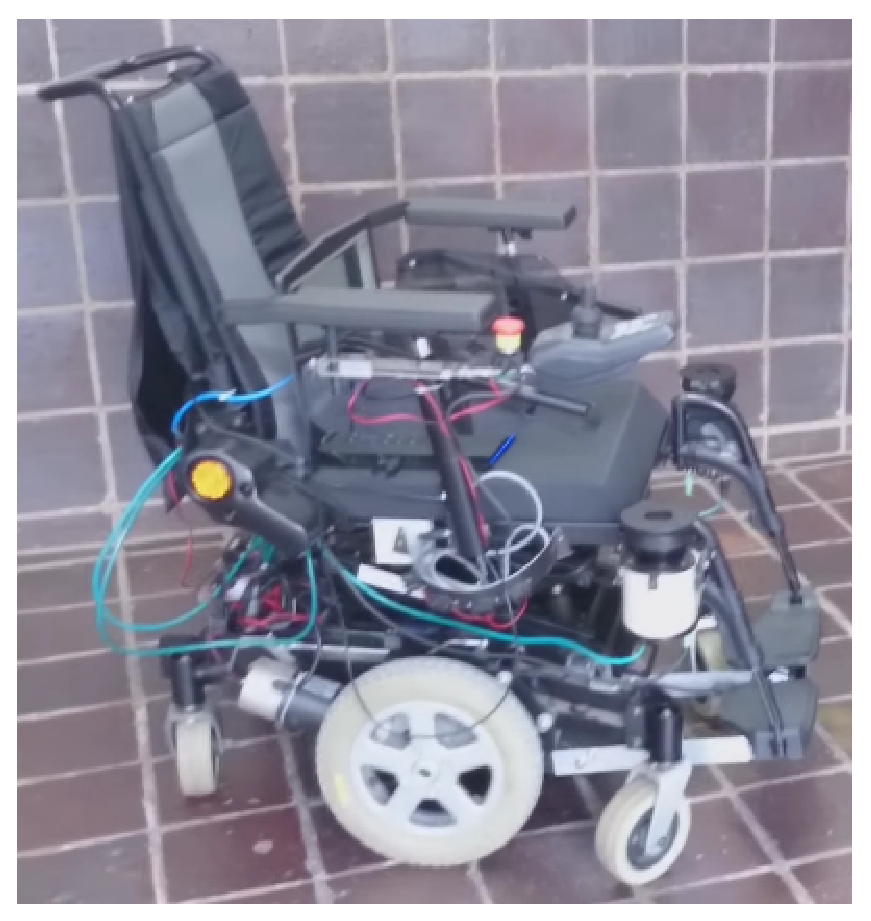
\includegraphics[width=0.48\textwidth]{images/cap3/Perenquen.eps}
  \end{center}
  \vspace{-20pt}
  \caption{Perenquén}
  \vspace{-10pt}
  \label{fig:Perenquen}
\end{wrapfigure}

El objetivo principal de este proyecto es el desplazamiento autónomo de una
silla de ruedas, mediante la detección de obstáculos de un entorno, así como su
localización en el mismo a través de las imágenes capturadas mediante la versión
2.0 de Kinect A diferencia de Verdino, Perenquén intenta ser una alternativa de
bajo coste frente a los sistemas de detección de obstáculo de Verdino.

Actualmente la silla cuenta con el dispositivo Kinect, un sistema de odometría
mecánica, y tres detectores láser (lado izquierdo, lado derecho y posterior) que
hacen posible una detección más precisa de los obstáculos. Sin embargo, Kinect
cuenta con una importante desventaja, y es que no funciona correctamente en
exteriores, tiene un alcance acotado de apenas entre 5 y 10 metros
\cite{PerenquenNoticia}.

%+++++++++++++++++++++++++++++++++++++++++++++++++++++++++++++++++++++++++++++++



%++++++++++++++++++++++++++++++++++++++++++++++++++++++++++++++++++++++++++++++
\section{ROS}
\label{3:sec3}
%%%%%%%%%%%%%%%%%%%%%%%%%%%%%%%%%%%%%%%%%%%%%%%%%%%%%%%%%%%%%%%%%%%%%%%%%%%%%%%%
% Chapter 3: Recursos y herramientas
%%%%%%%%%%%%%%%%%%%%%%%%%%%%%%%%%%%%%%%%%%%%%%%%%%%%%%%%%%%%%%%%%%%%%%%%%%%%%%%%

%+++++++++++++++++++++++++++++++++++++++++++++++++++++++++++++++++++++++++++++++
% \section{ROS}
% \label{3:sec:3}

% http://erlerobotics.com/blog/ros-introduction-es/
% https://www.clearpathrobotics.com/assets/guides/ros/Intro%20to%20the%20Robot%20Operating%20System.html
% http://www.ros.org/about-ros/

% http://www.ros.org/about-ros/
ROS (Robot Operating System) es un framework de código abierto diseñado para
realizar software robótico. Entre las principales funciondalidades destacan una
abstracción del hardware, el control de dispositivos, paso de mensajes entre los
procesos y una gran variedad de herramientas y librerías. Por otra parte ROS
cuenta con un sistema de paquetes, que permite instalar, compilar e incluso
modificar paquetes externos creados por la comunidad.

% http://erlerobotics.com/blog/ros-introduction-es/
El objetivo principal es permitir la abstracción y la simplifación de  muchas de
las tareas que conllevan construir un robot de forma independiente, uno de los
principales problemas que llevan a condenar al fracaso este tipo de proyectos,
mediante el desarrollo de software colaborativo. En definitiva, ROS promueve la
reutilización de código para evitar tener que reinventar la rueda a los
desarrolladores y científicos en cada nuevo proyecto.

% http://www.ros.org/about-ros/
De esta forma, a modo de ejemplo un grupo de desarrolladores puede trabajar e
investigar en la construcción de mapas, mientras que en otra parte del mundo,
otro grupo de expertos puede estar especializado en la localización con el uso
de mapas. Ambos comparten el conocimiento entre ambos y con el resto de la
comunidad para conseguir mejores resultados en conjunto.

% https://en.wikipedia.org/wiki/Robot_Operating_System
El software de ROS se distribuye de la siguiente manera:

\begin{itemize}
  \item Herramientas y lenguajes independientes para construir y distruibuir
  ROS.
  \item Librerías del cliente de ROS que facilitan el desarrollo.
  \item Paquetes que contienen la aplicación del usuario.
\end{itemize}

Tanto las herramientas como las librerías del cliente de ROS están escritas
principalmente en C++ y Python. Las librerías principales de ROS siguen los
principios Unix-like ya que la mayoría de dependencias son proyectos de código
abierto, permitiendo que muchas distribuciones distribuyan las librerías y
paquetes de ROS.

% http://www.ros.org/is-ros-for-me/
ROS ha sido diseñado para ser un sistema distribuido lo más modular posible,
permitiendo que los usuarios puedan utilizar lo justo y necesario, desde los
paquetes del núcleo y la comunidad, hasta utilizar sus propios paquetes
personales. Actualmente ROS cuenta con más de 3000 paquetes públicos en su
ecosistema, siendo difícil conocer cual es el número real de todos los paquetes.
Muchos de estos paquetes ayudan enormemente en la infraestructura de la
comunidad, ofreciendo accesos a drivers de dispositivo, capacidades genéricas en
robótica, algoritmos, herramientas de desarrollo y librerías.

Desde sus inicios, la comunidad de ROS ha crecido considerablemente en todo el
mundo, principalmente en laboratorios de investigación, pero en los últimos
tiempos también en otros sectores comerciales e industriales. Más de 1500
personas participan en las listas de correos, y aproximadamente 6000 personas
colaboran con la documentación oficial y la comunidad de preguntas y respuestas.
Esto implica que más de 30 páginas de la documentación se editen cada día y que
hasta la fecha se hayan abierto más de 13000 preguntas con un porcentaje de
respuesta alto.

%+++++++++++++++++++++++++++++++++++++++++++++++++++++++++++++++++++++++++++++++
\subsection{Historia}

% http://www.ros.org/about-ros/
El origen de ROS se remonta a 2007, cuando Willow Garage pensó en la necesidad
de de diseñar un sistema más flexivle y robusto para el desarrollo de robots
después de que en en el laboratorio de inteligencia artificial de la universidad
de Standford es estuvieran realizando diferentes proyectos que integraban el uso
de robots e inteligencia artificial como STandard AI Robot (STAIR) y Personal
Robots (PR).

% https://en.wikipedia.org/wiki/Robot_Operating_System
Varios investigadores contribuyeron y dieorn ideas para lo que sería la base
fundamental del servicio de paquetes de ROS que existe actualmente. En apenas un
año, el proyecto paso a desarollarse por la institución de investigación
robótica Willow Garage, junto con la colaboración de más de veinte
instituciones. Mientras tanto, el uso de una licencia permisiva de código
abierto permitió que de forma gradual ROS se empezará a implementar en
diferentes comunidades de desarrollo robótico. Finalmente, en 2013, ROS se
transferió a la Open Source Robotics Fundation.

Y hasta la fecha se han lanzado las siguientes versiones:

%+++++++++++++++++++++++++++++++++++++++++++++++++++++++++++++++++++++++++++++++
\begin{table}[!ht]
\begin{center}
\begin{tabular}{|p{50mm}|p{35mm}|p{60mm}|} \hline 
\textbf{Nombre} & \textbf{Lanzamiento} & \textbf{Soporte}\\ \hline
Kinectic Kame
&
23/05/2016
&
Soporte hasta 2021
\\
\hline

Jade Turtle
&
23/05/2015
&
Soporte hasta 2017
\\
\hline

Indigo Igloo
&
22/07/2014
&
Soporte hasta 2019
\\
\hline

Hydro Medusa
&
04/09/2013
&
Sin soporte
\\
\hline

Groovy Galapagos
&
31/12/2012
&
Sin soporte
\\
\hline

Fuerte Turtle
&
23/04/2012
&
Sin soporte
\\
\hline

Electric Emys
&
30/08/2011
&
Sin soporte
\\
\hline

Diamondback
&
02/03/2011
&
Sin soporte
\\
\hline

C Turtle
&
02/08/2010
&
Sin soporte
\\
\hline

Box Turtle
&
02/03/2010
&
Sin soporte
\\
\hline


\end{tabular}
\end{center}
\caption{Tabla con versiones de ROS hasta la fecha}
\label{table:playstation-camera}
\end{table}
%+++++++++++++++++++++++++++++++++++++++++++++++++++++++++++++++++++++++++++++++


%+++++++++++++++++++++++++++++++++++++++++++++++++++++++++++++++++++++++++++++++
\subsection{Infraestructura de ROS}
% http://www.ros.org/core-components/
% http://erlerobotics.com/blog/ros-introduction-es/#concepts
Uno de los elementos más básicos en la implementación de una aplicación robot es
el sistema de comunicación. ROS ofrece un sistema de mensajes entre los nodos
del sistema mediante un mecanismo que usa el patrón de publicación/suscripción.

Los nodos son los procesos que se encargan de las tareas concretas, como por
ejemplo controlar un láser, controlar los motores de las ruedas o planificar la
trayectoria del robot. Cada nodo tiene un nombre único en el sistema, para
evitar ambiguedad a la hora de comunicarse entre sí. Los nodos pueden ser
escritos en los diferentes lenguajes de las librerías del cliente de ROS (C++ o
Python por ejemplo).

% https://msdn.microsoft.com/es-es/library/ms152567(v=sql.120).aspx
Por otra parte, el patrón publicación/suscripción permite pasar información de
una manera sencilla y segura entre los nodos. En este patrón, existen dos
actores:

\begin{itemize}
  \item Publicador: publica la información.
  \item Suscriptor: recibe la información.
\end{itemize}

Una aproximación real de este patrón puede ser el editor de una revista. El
editor (publicador) escribe un número nuevo cada mes. Este número se distribuye
directamente o a través de un distribidor. En último lugar, tenemos a una
persona suscrita a esa revista (suscriptor), a quien le llega cada mes un nuevo
número de la revista.

La información que se intercambian los nodos (en el ejemplo anterior los
ejemplares de la revista) se conoce como mensaje. Un mensaje es una estructura
con una serie de campos primitivos: enteros, flotantes, booleanos, cadenas de
texto, etc.

Para el intercambio de información entre los nodos, los mensajes deben
transmitirse por un canal, en este caso denominado tópico. Los tópicos utilizan
un nombre para describir el contenido de los mensajes, por lo que, un tópico
transmite un cierto tipo de datos. Si un nodo desea recibir cierto tipo de
datos, se debe suscribir al tópico apropiado del nodo. Por ejemplo una cámara y
un visor, ambos comparten el tópico 'imagen', cada vez que la cámara captura una
imagen el resultado se publica (publicador), si el visor espera recibir una
imagen y está suscrito al tópico 'imagen' de la cámara, esta se transmitirá. Un
nodo puede publicar o suscribirse a múlitples tópicos, además, pueden haber
muchos publicadores concurrentemente para un sólo tópico.

Una de las mayores ventajas del sistema de publicación/suscripción es que es
anónimo y asíncrono, por lo que los mensajes que se transmiten no se modifican.
Sin embargo, a veces es necesario realizar comunicaciones entre los nodos de
manera síncrona o mediante interacciones de petición y respuesta en vez de
realizar el transporte de los mensajes en un ún único sentido. Para ello, ROS
ofrece lo que se llaman servicios. La petición y respuesta se definen mediante
una estructura de mensajes, una para la petición y otra para la respuesta.

% http://answers.ros.org/question/11834/when-should-i-use-topics-vs-services-vs-actionlib-actions-vs-dynamic_reconfigure/
Es necesario conocer, que los tópicos se usan cuando se desea transmitir
mensajes que continuamente envían información (datos de los sensores, estado del
robot, imágenes capturadas, etc.), mientras que los servicios están pensados
para realizar una petición y recibir una respuesta bajo demanda en ocasiones
concretas.

% SERVIDOR D EPARAMETROS
Por otra parte, ROS utiliza lo que se conoce como servidor de parámetros, un
diccionario compartido de clave-valor y accesible desde la red. Los nodos usan
el servidor para almacenar y recibir parámetros en tiempo de ejecución, y de
esta forma modificar el funcionamiento del sistema.

ROS cuenta con las herramientas para monitorizar y controlar el estado de los
nodos, tópicos, servicios y parámetros mediante 'rosnode', 'rostopic',
'rosservice' y 'rosparam'. Para que el sistema funcione correctamente, es
necesario que este activo el ROS Master. Se trata del nodo maestro, sin él los
nodos no podrían encontrar al resto de nodos, tampoco se podría intercambiar
mensajes o invocar servicios.

En la figura ~\ref{fig:Ros-Diagram} se puede observar una implementación de como
captura imágenes un robot. Por un lado existen tres nodos: el nodo de la cámara
que recibe de la cámara, y los nodos de procesamiento de las imágenes y la
visualización de las mismas. Estos dos nodos están suscritos al tópico
'/image-data' que publica el nodo de la cámara. Cada vez que la cámara registra
una nueva imagen se transmite a los otros nodos.

\begin{minipage}{\linewidth}
    \centering
    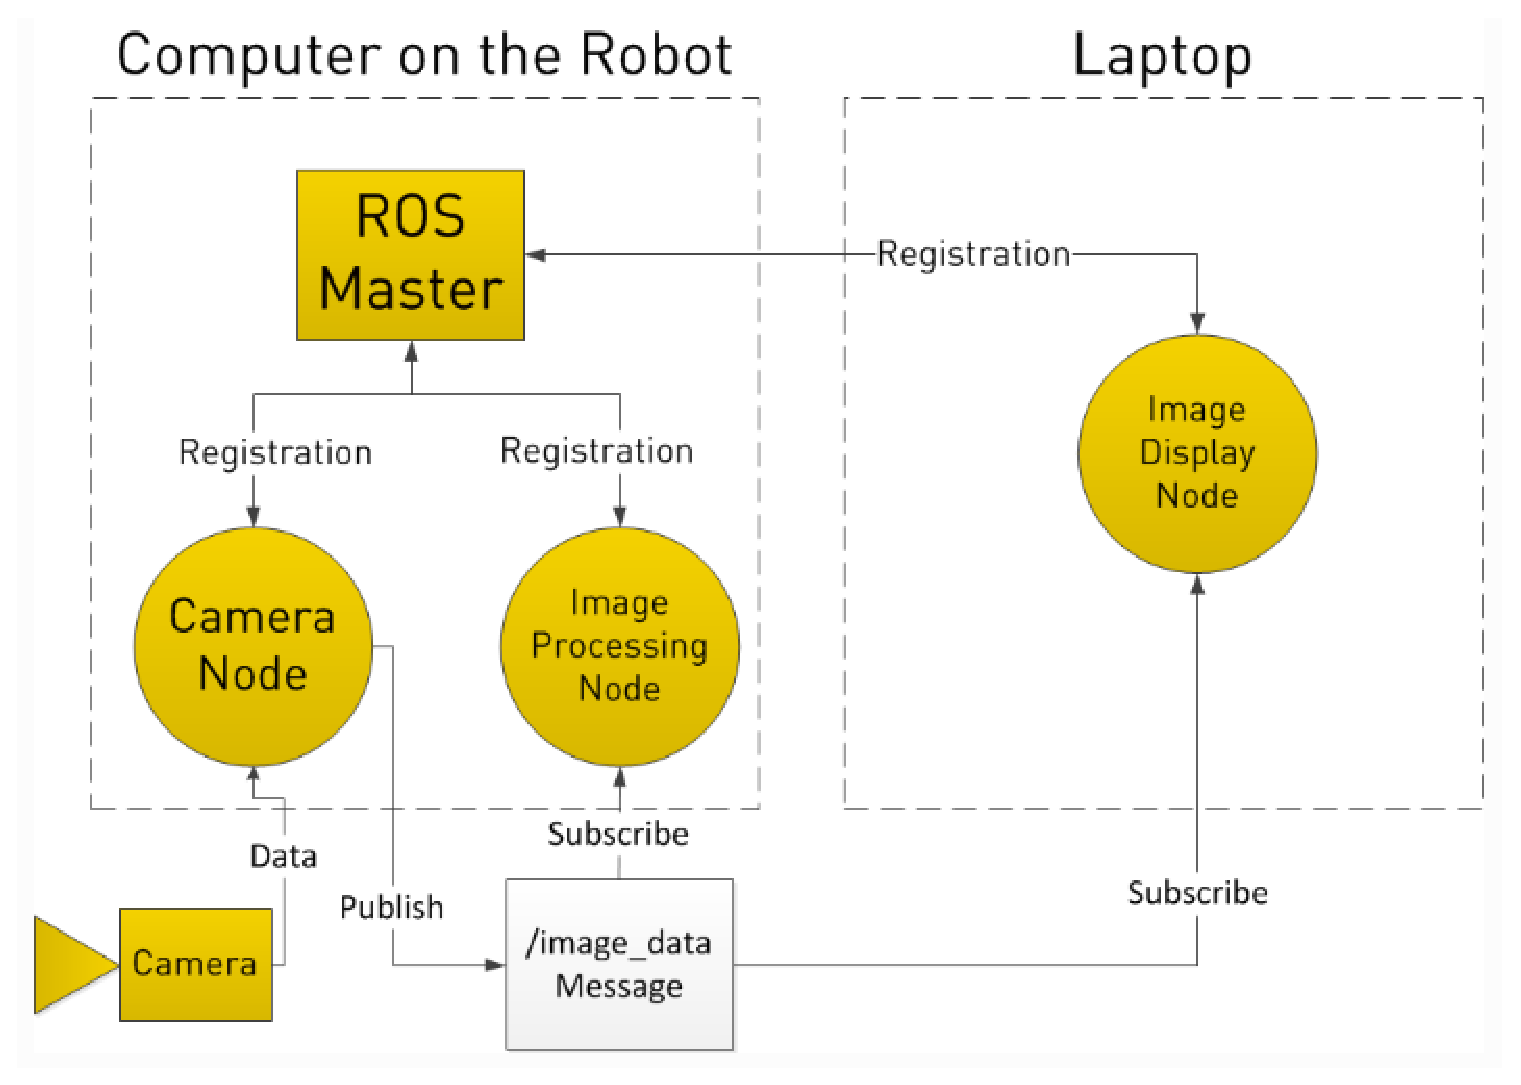
\includegraphics[width=0.8\textwidth]{images/cap3/RosDiagrama.eps}
    \captionof{figure}{Ejemplo de captura de imágenes}
    \label{fig:Ros-Diagram}
\end{minipage}

%+++++++++++++++++++++++++++++++++++++++++++++++++++++++++++++++++++++++++++++++
\subsection{Características}
% http://www.ros.org/core-components/

%+++++++++++++++++++++++++++++++++++++++++++++++++++++++++++++++++++++++++++++++
\subsection{Herramientas}
% http://www.ros.org/core-components/
Una de las características más importatnes de ROS está en las herramientas de
desarrollo disponibles. Existe una gran variedad de software de todo tipo:
visualización, depuración, resumen del estado, etc. Gracias al mecanismo de
publicación/suscripción es muy sencillo observar y depurar lo que está
ocurriendo en todo momento.

Por otra parte, ROS puede ser utilizado sin necesidad de usar una interfaz
gráfica (GUI). Toda las características y funcionalidades de ROS pueden
realizarse a través de más de 45 comandos en consola: lanzar grupos de nodos,
examinar tópicos y servicios, grabar y reproducier bolsas de datos, etc. En
cualquier otro caso existe una importante variedad de herramientas con interfaz
gráfica que extienden la funcionalidad de estos comandos. A continuación se
pueden ver algunos de ellos.

%--------------------------------------
\paragraph{RTAB-Map} \hspace{0pt}

Construir el mapa, que mas quieres

%--------------------------------------
\paragraph{RViz} \hspace{0pt}

RViz es una herramienta de propósito general que permite visualizar en un
espacio tridimensiona mucho de los elementos de un robot como ruedas, brazos o
sensores láser. RViz también puede visualizar diferentes mensajes comúnes de ROS
como barridos láser, nube de puntos, las imágenes de las cámaras o también con
la posibilidad de mostrar el mapa del entorno (previamente almacenado).

RViz también puede interactuar con la información de la biblioteca 'tf' para
mostrar toda la información del sistema de coordenadas de los sensores desde
diferentes perespectivas. Entre las ventajas, destaca que se trata de una
herramienta muy importante ya que permite visualizar que ocurre en el robot en
cada momento en busca de errores.

%--------------------------------------
\paragraph{RQt} \hspace{0pt}

%+++++++++++++++++++++++++++++++++++++++++++++++++++++++++++++++++++++++++++++++
\subsection{4}

